\subsection*{ГЛ11 8}
\begin{figure}[h]
	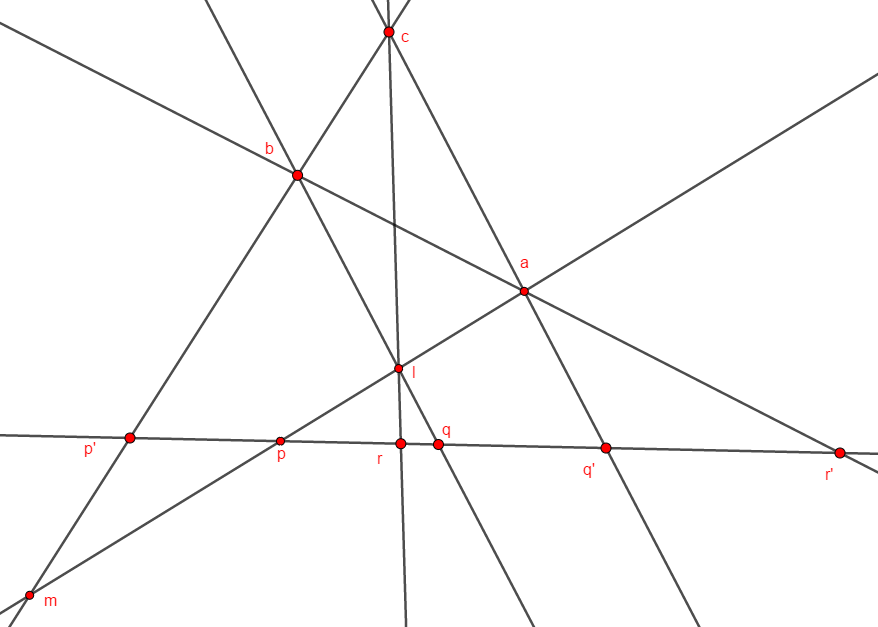
\includegraphics[width=0.5\linewidth]{pic9}
\end{figure}
Докажем от противного. Тогда $l \notin (cr)\quad (bq) \cap (ap) = l$\\
Заметим, что проективное преобразование одной прямой в другую однозначно задается по трем точкам (то есть по 3 точкам на одной прямой и их образами на другой)\\		
Пусть $f_1: \mathbb{R}\text{P}^2 \to \mathbb{R}\text{P}^2|\ [p'pqr'] = [mpla]$ при этом $(p'm) \cap (ql) \cap (r'a) = b$\\
И $f_2: \mathbb{R}\text{P}^2 \to \mathbb{R}\text{P}^2|\ [mpla]= [p'pr_0q']$ при этом $(mp') \cap (lr_0) \cap (aq') = c,\ r_0 = (cl) \cap (p'r')$\\
$[p'pqr'] = [p'pr_0q'] \rightarrow [pp'r'q] = [p'pr_0q']$\\
Если в проективном преобразовании $f$ существуют 2 различные точки для которых $f(a) = b, f(b) = a$, то $f$ -- инволюция\\
$f_3:\ [pp'r'q] = [p'pr_0q]$ -- инволюция, следовательно $r'\to r_0 \ne r$, откуда следует, что либо $l \in (cr),\ (bq) \cap (ap) \cap (cr) = l$, либо такой инволюции $f_3: l \to l$ не существует.\\
Заметим, что каждая из прямых проводилась либо случайныиобразом, либо в точку пересечения двух других, следовательно если какую-то из прямых мы не можем провести(из-за малой длины линейки), то мы можем применить аналогичное построение уже для новой пары точек.
